\section{Queue (Coda)}
Le code sono delle strutture dati con organizzazione {\textbf{FIFO}}
(First-In-First-Out).
Possono essere implementate tramite array o tramite liste concatenate. Sono 
preferibili le liste doppiamente concatenate.\newline
\begin{wrapfigure}{r}{7cm}
    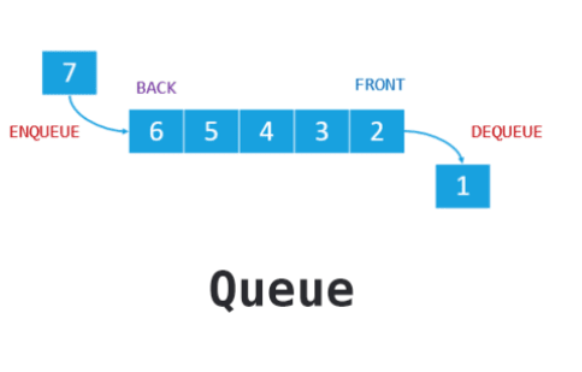
\includegraphics{queue.png}
\end{wrapfigure}

Le operazioni che possono essere eseguite su una coda sono:
\begin{itemize}
    \item {\texttt{isEmpty() $\rightarrow$ boolean}} restituisce \verb|true| se la coda è vuota, \verb|false| altrimenti
    \item {\texttt{enqueue(elemento)}} aggiunge un elemento alla coda
    \item {\texttt{dequeue() $\rightarrow$ elemento}} rimuove il primo elemento dalla coda e lo restituisce
    \item {\texttt{first() $\rightarrow$ elemento}} restituisce il primo elemento della coda
\end{itemize}

\begin{algorithm}
    \caption{isEmpty}
    \Indm{\textbf{Funzione}} {\emph{isEmpty}}() $\rightarrow$ {\emph{boolean}}\\
       \Indp\eIf{$primo = null$}{\Return{$true$}}{\Return{$false$}}
\end{algorithm}

\begin{algorithm}
    \caption{first}
    \Indm\textbf{Funzione} \emph{first}() $\rightarrow$ elemento\\
    \Indp\Return{$primo.dato$}
\end{algorithm}

\begin{algorithm}
    \caption{dequeue}
    \Indm\textbf{Funzione} \emph{dequeue}() $\rightarrow$ elemento\\
    \Indp$x$ $\leftarrow$ $primo.dato$\\
    $primo$ $\leftarrow$ $primo.pros$\\
    \If{$primo = null$}{$ultimo \leftarrow null$}
    \Return{$x$}
\end{algorithm}

\begin{algorithm}
    \caption{enqueue}
    \Indm\textbf{Procedura} \emph{enqueue}(elemento \emph{x})\\
    \Indp$r$ $\leftarrow$ riferimento ad un nuovo nodo\\
    $r.dato$ $\leftarrow$ $x$\\
    $r.pros$ $\leftarrow$ $null$\\
    \eIf{$primo = null$}{
        $primo \leftarrow r$\\
        $ultimo \leftarrow r$
    }{
        $ultimo.pros \leftarrow r$\\
        $ultimo \leftarrow r$
    }
    
\end{algorithm}


\clearpage